\documentclass[border=0.2cm]{standalone}

\usepackage{tikz}
\usetikzlibrary{shapes.geometric, shapes.misc}
\usetikzlibrary{cd, fit, calc}
\usetikzlibrary{positioning}
\usetikzlibrary{decorations.markings, decorations.pathreplacing}
\usepackage{medl_colors}
\usepackage{ifthen}

\graphicspath{ {./images/} }

\newcommand{\fetchitem}[2]{
  \foreach \x [count=\k] in #1 {
        \ifnum\k=#2
            \x
        \fi
    }
}
\newcommand{\recursiveRectangleZero}[6]{
  \node (rect) at (#1,#2) [draw,#4,rounded corners,minimum width=0.9cm,minimum height=3cm] (#61)  {$\fetchitem{{#5}}{3}$};
  \foreach \i in {2,...,#3} {
       \node (rect)[draw,#4,rounded corners,minimum width=0.9cm,minimum height=3cm,right of=#61,node distance={(\i-1)*3.1cm}] (#6\i)  {$z_{\fetchitem{{#5}}{\i}}$};
       \pgfmathtruncatemacro{\prevIndex}{\i - 1};
       \draw [Triangle-, thickline] ($(#6\i.west)+(0,1)$) --  ($(#6\prevIndex.east)+(0,1)$) node[above,pos=0.5,font=\small]{$q_{\phi_{\fetchitem{{#5}}{\prevIndex}}}(z_{\fetchitem{{#5}}{\i}} |  \fetchitem{{#5}}{3})$};
       \draw [Triangle-, thickline] ($(#6\prevIndex.east)+(0,-1)$) -- ($(#6\i.west)+(0,-1)$)node[below,pos=0.5,font=\small]{$p_{\theta_{\fetchitem{{#5}}{\i}}}(\fetchitem{{#5}}{3} | z_{\fetchitem{{#5}}{\i}})$};
  }
}
\newcommand{\recursiveRectangle}[6]{
  \node (rect) at (#1,#2) [draw,#4,rounded corners,minimum width=0.9cm,minimum height=3cm] (#61)  {$z_{\fetchitem{{#5}}{1}}$};
  \foreach \i in {2,...,#3} {
       \node (rect)[draw,#4,rounded corners,minimum width=0.9cm,minimum height=3cm,right of=#61,node distance={(\i-1)*3.1cm}] (#6\i)  {$z_{\fetchitem{{#5}}{\i}}$};
       \pgfmathtruncatemacro{\prevIndex}{\i - 1};
       \draw [Triangle-, thickline] ($(#6\i.west)+(0,1)$) --  ($(#6\prevIndex.east)+(0,1)$) node[above,pos=0.5,font=\small]{$q_{\phi_{\fetchitem{{#5}}{\prevIndex}}}(z_{\fetchitem{{#5}}{\i}} |  z_{\fetchitem{{#5}}{\prevIndex}})$};
       \draw [Triangle-, thickline] ($(#6\prevIndex.east)+(0,-1)$) -- ($(#6\i.west)+(0,-1)$)node[below,pos=0.5,font=\small]{$p_{\theta_{\fetchitem{{#5}}{\i}}}(z_{\fetchitem{{#5}}{\prevIndex}}| z_{\fetchitem{{#5}}{\i}})$};
  }
}

\newcommand{\customArrow}[5]{
    \ifthenelse{\equal{#5}{right}}{%
         \draw[dashed, uthickline] (#1,#2) -- (#3-1,#4);
         \draw[-Triangle, thickline] (#3-0.9,#4) -- (#3,#4) {};
    }{
         \draw[dashed, uthickline] (#1,#2) -- (#3+1,#4);
         \draw[-Triangle, thickline] (#3+0.9,#4) -- (#3,#4) {};
    }
}

\begin{document}
\begin{tikzpicture}

\recursiveRectangleZero{0}{0}{2}{blueshape}{0, 1, x}{id1};
\recursiveRectangle {7.7}{0}{3}{blueshape}{{t-1},{t},{t+1}}{id2}(ring2);
\recursiveRectangle {18.5}{0}{2}{blueshape}{{\scriptscriptstyle T-1},{\scriptscriptstyle T}}{id3};

\customArrow{3.55}{1}{7.2}{1}{right};
\customArrow{7.2}{-1}{3.55}{-1}{left};
\customArrow{14.35}{1}{18.0}{1}{right};
\customArrow{18.0}{-1}{14.35}{-1}{left};

\node[below right = 2cm and -1cm of id11, scale = .4] (pica) {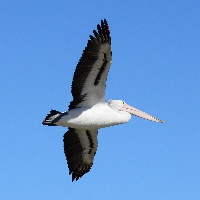
\includegraphics {images/noisy_image_00.jpg}};
\node[below left = 2cm and -1.9cm of id22, scale = .4] (picb) {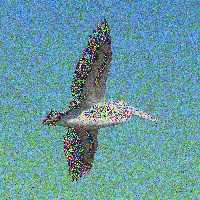
\includegraphics {images/noisy_image_03.jpg}};
\node[below right = 2cm and 0.3cm of id31, scale = .4] (picc) {
\includegraphics {images/noisy_image_10.jpg}};

\draw [-Triangle, bthickline] ($(picb.north)+(-2.5,6)$) -- ($(picb.north)+
(2.5,6)$) node[above, midway](de3){\large {Encoder}};
\draw [Triangle-, bthickline] ($(picb.south)+(-2.5, 4)$) -- ($(picb.south)+ (2.5, 4)$) node[below, midway](de3){\large {Decoder}};

\end{tikzpicture}
\end{document}
